\documentclass[../main.tex]{subfiles}

\begin{document}
% subsecciones de ejemplo, no es necesario seguir esta estrctura

La realidad virtual es una de las tecnologías que más ha avanzado en los últimos años. Estos avances han permitido que se pueda aplicar a sectores como la medicina, la psicología, los videojuegos, o incluso la educación. Gran parte de su fama es adquirida gracias a los videojuegos, que llevan los entornos tridimensionales a otro nivel, permitiendo aumentar las sensaciones que perciben los usuarios, como el miedo o el vértigo, e incluso permiten que un usuario se relaje, disminuyendo su estrés. Haciendo uso de motores gráficos como Unity, los desarrolladores pueden crear multitud de entornos virtuales para diferentes propósitos y sectores.

Para simular estos entornos y poder verlos e interactuar con ellos, son necesarios dispositivos como gafas de realidad virtual o mandos, entre otros. Gracias a estos dispositivos es posible conseguir que los usuarios sientan que forman parte del entorno, ya que lo perciben de manera prácticamente indistinguible de la realidad y pueden interactuar con muchos de los elementos que lo forman.

La llegada de la realidad virtual supone uno de los avances tecnológicos que más cambian el enfoque de los usuarios. Estos avances cambian por completo la percepción que tiene el usuario y la manera en la que interactúa con distintos sistemas o la forma en la que recibe información o estímulos. Además permiten, en cierta medida, transportar al usuario al entorno deseado evadiendo la realidad, haciendo incluso que olvide que está limitado por el entorno del mundo real.

%%Imagen del Sensorama, centrada y con el caption
\begin{figure}[htbp]
\centering
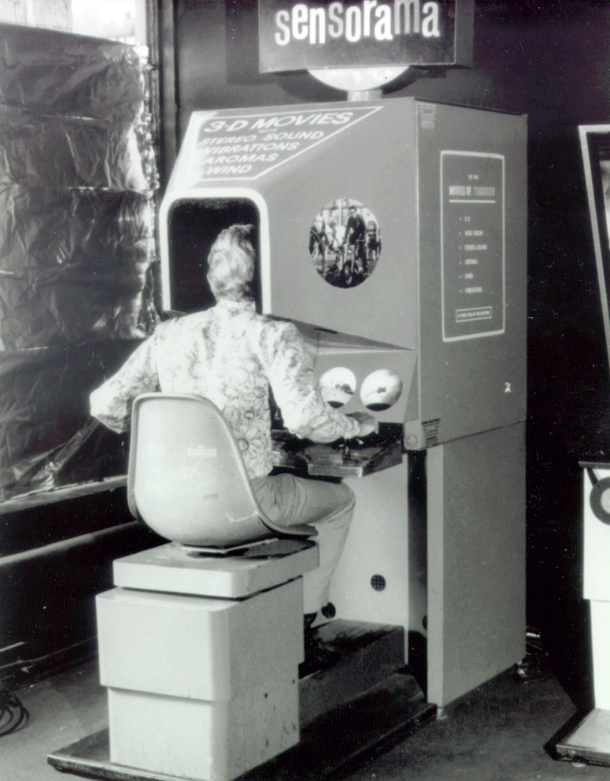
\includegraphics[width=5cm, height= 5cm]{imagenes/Sensorama.jpg}
\caption{Sensorama. Fuente:\cite{Sensorama}}
\label{fig:Sensorama}
\end{figure}

No obstante, la realidad virtual no ha tenido tanta fama en el pasado. El primer prototipo de un sistema de realidad virtual fue diseñado por Morton Heilig, en los años 1960-1962, y lo llamó Sensorama (Ver figura \ref{fig:Sensorama}). Este sistema mostraba un espacio en realidad virtual pero, al ser la primera aproximación a esta tecnología, carecía de interacción con el entorno.

Esta máquina ofrecía una experiencia cinematográfica inmersiva, que simulaba también algunos aspectos como el viento o el olor del entorno tal y como explican Tomasz Mazuryk y Michael Gervautz \cite{Tomasz_Michael}.

La aplicación de realidad virtual en videojuegos empieza en el año 1995, teniendo aún un largo camino por delante, en su mayoría abocado al fracaso. Nintendo lanza al mercado la Virtual Boy (Ver figura \ref{fig:Virtual_Boy}), que fue el primer prototipo comercial de gafas de realidad virtual, que utiliza en su interior un proyector para mostrar imágenes tridimensionales mediante efectos estereoscópicos. Su comercialización, así como la de multitud de dispositivos de otras compañías, fue un fracaso debido a la incómoda postura que había que adoptar para utilizarlas y las dificultades para publicitarlas entre otras cosas.

%%Imágen de la Virtual BOY, centrada y con el caption
\begin{figure}[htbp]
\centering
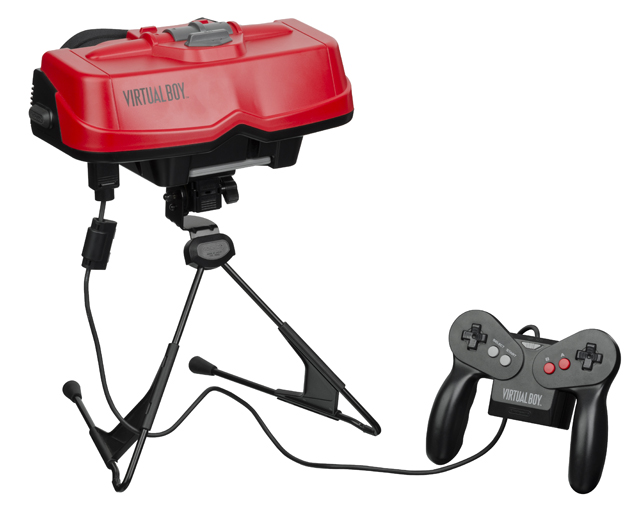
\includegraphics[width=5cm, height= 4.2cm]{imagenes/Virtual_Boy.jpg}
\caption{Virtual Boy de Nintendo. Fuente:\cite{VirtualBoy}}
\label{fig:Virtual_Boy}
\end{figure}

En el año 2010 se crea el primer prototipo de dispositivo de realidad virtual de Oculus Rift, que se convirtió con el paso de los años en uno de los referentes en la industria. Las nuevas mejoras y funcionalidades que ofrece este dispositivo suponen un cambio en el enfoque a la realidad virtual en general. En este momento el usuario que utiliza las gafas, deja de encontrarse en el espacio de manera pasiva, para empezar a explorar entornos e interactuar con sus elementos de manera activa. 

%%Imágen de las Oculus Rift DK1
\begin{figure}[htbp]
\centering
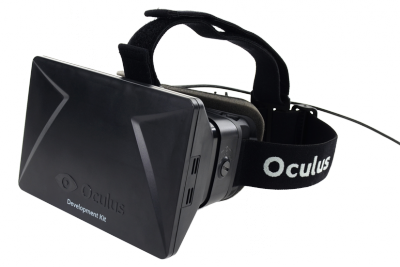
\includegraphics[width=5cm, height= 3.5cm]{imagenes/Oculus_Rift_DK1.png}
\caption{Oculus Rift DK1. Fuente:\cite{OculusDK1}}
\label{fig:OculusDK1}
\end{figure}

\clearpage
Los nuevos dispositivos y sus diferentes accesorios aumentan en gran cantidad la sensación de presencia en el espacio, lo que hace que aumente su popularidad y empiece a utilizarse en muchos otros sectores.

Existen multitud de utilidades y funcionalidades de los nuevos dispositivos de realidad virtual en la actualidad que pueden aplicarse a múltiples industrias, gracias a esta sensación de inmersión mejorada que es posible conseguir. Un ejemplo clave son las simulaciones virtuales, que se aplican, por ejemplo, para entrenar profesionales de diferentes ámbitos. Algunos ejemplos serían las simula- ciones utilizadas para aprendizaje práctico de oftalmólogos \cite{VR_Oftalmology} o entrenamiento de combate de militares \cite{VR_Military}.

También es posible tratar problemas cognitivos, sensoriales o incluso traumas psicológicos. Por ejemplo, para rehabilitar a personas con problemas de equilibrio e historiales de caídas extensos, se proponen entrenamientos en cintas de correr en realidad virtual \cite{VR_Cognitive}, y para tratar el trastorno de estrés postraumático que sufren las víctimas de accidentes de tráfico, se crean situaciones de conducción a tiempo real \cite{VR_PTSD}. Estos son solo algunos ejemplos de la infinidad de aplicaciones que tiene la realidad virtual en la actualidad.

Este tipo de investigaciones ha revelado la gran eficacia de la aplicación de la realidad virtual ayudando a las personas a superar algunos traumas o trastornos y a mejorar muchas habilidades mediante el entrenamiento en entornos virtuales gracias a la sensación de inmersión conseguida.

No obstante, un problema muy recurrente es la limitación en el espacio de trabajo que hay disponible, ya que para llevar a cabo algunas investigaciones o experimentos en ocasiones se necesita más espacio que el que se tiene disponible, o es necesario que el usuario se desplace por el entorno virtual sin que el real sea una limitación. Un ejemplo muy claro es el de los videojuegos, para conseguir una sensación de presencia en el entorno virtual lo mayor posible, lo ideal sería que el usuario se desplazase por el entorno virtual igual que lo hace en el mundo real, andando o corriendo. Este tipo de movimiento en realidad virtual se conoce como \textit{Room Scale} \cite{RoomScale}, y se encarga de hacer una correspondencia exacta entre el movimiento físico del usuario y el movimiento en el entorno virtual.

Para conseguir este efecto, se utilizan multitud de técnicas para que el movimiento se sienta real. Un ejemplo claro es el movimiento mediante teletransporte, que es la única técnica de locomoción no continua, es decir, la única donde el usuario pasa de estar en un punto a otro instantáneamente, sin camino entre medias. El usuario selecciona el punto donde quiere llegar con el mando y después es teletransportado. Como explica Arthur Ribeiro \cite{Teletransport_Movement}, existen 2 tipos de teletransporte. Al primero se la llama parpadeo, y es el que hemos explicado anteriormente, y el segundo es el llamado desplazamiento. Este último se diferencia del parpadeo en que no es instantáneo, sino que hay un rápido movimiento entre el punto inicial y el final, que da sensación al usuario de que se hace el recorrido completo. Este tipo de movimiento evita los posibles mareos que los usuarios pudiesen tener al utilizar un dispositivo de realidad virtual.

Sin embargo, aplicar tanto esta técnica como otras basadas en movimiento lineal mediante un mando en ocasiones no es posible. Para estas situaciones, existen algunas soluciones que permiten al usuario desplazarse de manera intuitiva por el entorno, como por ejemplo el sistema Omni One, que se muestra en la figura \ref{fig:Omni_One}. Este sistema hace uso de una base a los pies del usuario que funciona como una cinta de correr, lo que permite que pueda moverse sin desplazarse realmente en el mundo real mientras traduce sus movimientos al juego. También utiliza un arnés que permite que el jugador pueda rotar 360 grados y mantenerlo en el centro de la base.

%%Imágen de la Omni One
\begin{figure}[htbp]
\centering
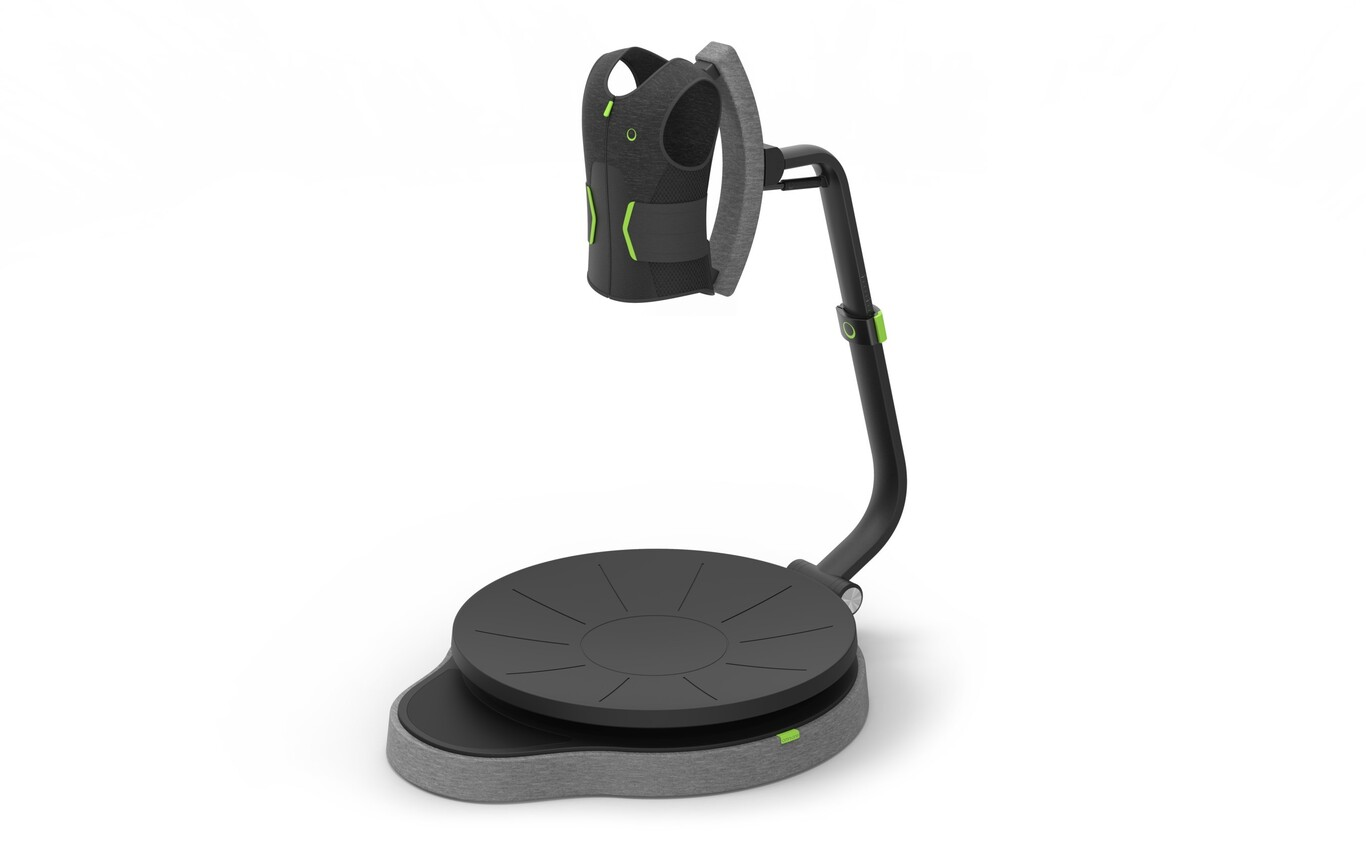
\includegraphics[width=10cm, height= 6cm]{imagenes/Onmi_One.jpeg}
\caption{Sistema Omni One. Fuente:\cite{OmniOne}}
\label{fig:Omni_One}
\end{figure}

Aunque este tipo de sistemas solucionan de manera efectiva el problema, hay que tener en cuenta que son muy complejos y llegan a costar cantidades que no todos los usuarios están dispuestos a pagar.

En este proyecto se busca crear un sistema que permita generar laberintos procedimentales aprovechando el espacio de trabajo gracias a los espacios no euclidianos, superponiendo las diferentes secciones del laberinto. Para conseguirlo, haremos uso de un efecto visual que funciona como un portal adaptado a realidad virtual \cite{TFG_David}, de manera que es posible teletransportar a un usuario de un espacio determinado a otro con unas características completamente diferentes creando así distintos espacios que rompen con los postulados de Euclides que se explican más adelante.


Para poder comprender este efecto y cómo puede afectar a la experiencia del usuario, primero se necesita conocer qué es la geometría euclidiana y los cinco postulados que estableció Euclides en el tratado denominado Los Elementos \cite{Euclides}, escrito en el año 300 a.C., que a pesar de ser un trabajo sobre geometría, incluye resultados calificables dentro de la teoría de números. Estos cinco postulados son los siguientes:

\begin{itemize}
    \item \textbf{1.} Se podrá dibujar un segmento de recta entre dos puntos cualesquiera.
    \item \textbf{2.} Un segmento de recta se puede extender indefinidamente en una línea recta.
    \item \textbf{3.} Se puede trazar una circunferencia dados un centro y una distancia desde ese centro.
    \item \textbf{4.} Todos los ángulos rectos son iguales entre sí.
    \item \textbf{5.} Si una recta corta a otras dos formando dos ángulos internos agudos por un mismo lado, esas dos rectas prolongadas indefinidamente se cortarán del lado en el que están dichos ángulos (Ver figura \ref{fig:5th_postulate}).
\end{itemize}

%%Imagen del quinto postulado de Euclides
\begin{figure}[htbp]
\centering
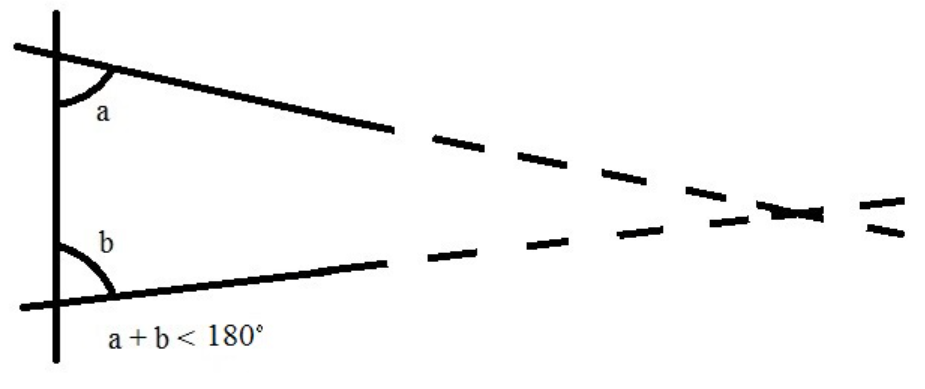
\includegraphics[width= 10cm, height= 4.5cm]{imagenes/5th_euclid_postulate.png}
\caption{El quinto postulado de Euclides. Fuente:\cite{5th_postulate}}
\label{fig:5th_postulate}
\end{figure}

La geometría que se utiliza en el desarrollo de este proyecto pretende vulnerar parcial o momentáneamente estos principios geométricos, representando espacios virtuales más amplios superponiendo la geometría dentro de un mismo espacio de trabajo disponible.

\section{Planteamiento del problema}

Como se explica anteriormente, la tecnología de la que disponemos actualmente permite conseguir que los usuarios se sientan completamente inmersos en los entornos virtuales, de manera que, en muchos casos, se olviden por completo del entorno real y se desplacen sin tenerlo en cuenta.

Aunque en el pasado muchos desarrolladores han llevado a cabo técnicas ingeniosas para evadir este problema, si lo que se busca es una sensación de presencia completa, una buena solución es la utilización de espacios parcialmente no euclidianos. Por lo tanto en este proyecto haremos uso de estos espacios para poder crear entornos que un usuario pueda recorrer con un espacio de trabajo limitado sin necesidad de utilizar sistemas complejos.

Uno de los objetivos principales del proyecto es poder explorar entornos lo más grandes posibles, y, por lo tanto debe ser posible generar espacios prácticamente infinitos de forma que sus características sean aleatorias mientras no se excedan los límites del espacio de trabajo. Para ello, es necesario almacenar todo el entorno virtual generado en una estructura de datos sobre la que se tenga control total, de manera que se puedan cargar las partes necesarias en cada momento.

Para conseguir infinidad de entornos diferentes que explorar, se hará uso de algoritmos procedimentales, de manera que sea posible crear espacios de caracte- rísticas aleatorias que cumplan una serie de condiciones que mantengan la integridad del entorno.

Con la generación de estos escenarios se pretende crear una solución a la limitación que supone el espacio de trabajo al utilizar como método de desplazamiento \textit{Room Scale}, consiguiendo así que un usuario pueda explorar infinidad de entornos de dimensiones potencialmente infinitas mientras sigue inmerso en el entorno virtual y se olvida completamente del espacio real del que dispone.

\section{Objetivos} \label{Objectives}

Para organizar todo el trabajo necesario para conseguir el resultado deseado, se divide el trabajo en las siguientes fases:

\begin{itemize}
    \item 1. Adaptar el efecto del portal existente al nuevo sistema de Unity.
    \item 2. Crear una estructura de datos que permita almacenar toda la información del laberinto así como las características de sus secciones.
    \item 3. Diseñar un sistema que permita renderizar cualquier sección del laberinto a partir de sus características.
    \item 4. Calcular las características de las diferentes secciones del laberinto teniendo en cuenta la posición del jugador y los posibles movimientos que este puede hacer, para mantenerlo siempre dentro de los límites del espacio de trabajo.
    \item 5. Conectar coherentemente las secciones del laberinto mediante los portales.
\end{itemize}

Una vez conseguidos estos objetivos se espera disponer de un sistema que permita generar espacios de una longitud específica cuyas características sean aleatorias de manera que un usuario pueda recorrer cualquier punto sin salirse de los límites que supone el entorno real gracias a la utilización de entornos parcialmente no euclidianos, y preservando en todo momento la sensación de inmersión en el entorno virtual gracias a los dispositivos de realidad virtual.

\section{Estructura del documento}

Una vez se han planteado los objetivos del proyecto y el problema que se intenta solucionar, se expone a continuación la estructura del documento de manera que se facilite el seguimiento del documento.

\begin{itemize}
    \item En el Capítulo 2 se trata el Estado del arte. En este apartado se expone la situación actual de los diferentes sistemas, técnicas y tecnologías de las que se hace uso a lo largo del desarrollo del proyecto.
    \item En el Capítulo 3 se expone el Desarrollo. En este apartado se encuentran explicados todos los pasos que se han realizado desde el inicio del proyecto hasta la obtención del resultado. En él, se explica con detalle la función de cada clase implementada y la lógica detrás de ella.
    \item En el Capítulo 4 se muestra el Resultado. Se exponen los resultados conseguidos al terminar el desarrollo del proyecto mostrando diferentes ejemplos para que el lector comprenda su utilidad.
    \item En el Capítulo 5 se exponen las Conclusiones y Trabajos Futuros. En este punto se reflexiona sobre toda la información del documento con el fin de extraer la información e ideas esenciales. Se analiza también el impacto que el proyecto pudiese tener tanto social como ambientalmente y se termina proponiendo ideas y proyectos en los que se pueda continuar tratando el tema de este Trabajo de Fin de Grado.
\end{itemize}

\end{document}